\documentclass[12pt]{article}
\usepackage[utf8]{inputenc}
\usepackage{amssymb,amsmath}
\usepackage{hyperref}
\usepackage{graphicx}
\author{Claas Jaehrling, Sven-Hendrik Haase}
\title{RS1 HA zum 16.12.11}
\date{\today}
\begin{document}
\setcounter{secnumdepth}{0}
\maketitle

\section{Aufgabe 8.1}
\subsection{(a)}
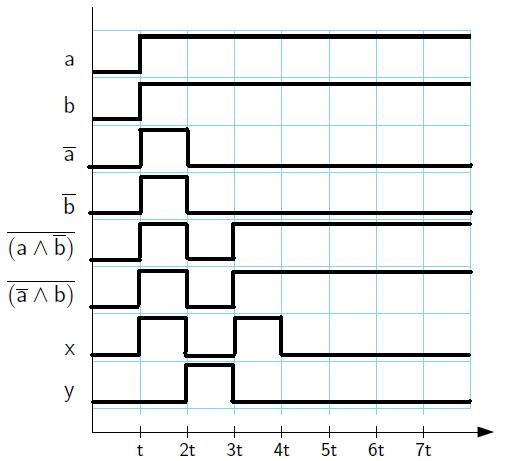
\includegraphics{Impulsdiagramm81a}\\
Als Folge von Strukturhazards tritt ein dynamischer 1-Hazard am Ausgang x auf.
\subsection{(b)}
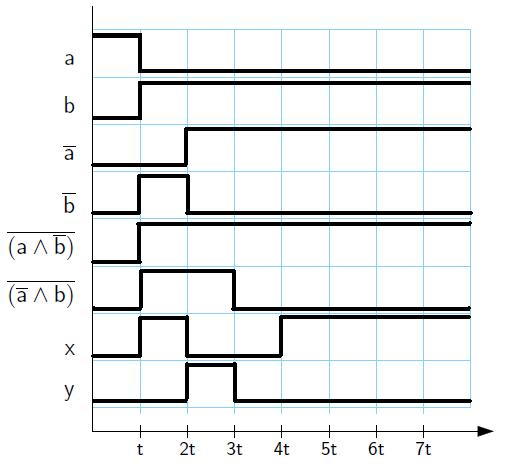
\includegraphics{Impulsdiagramm81b}\\
Als Folge von Strukturhazards tritt ein dynamischer 0-Hazard am Ausgang x auf.
\section{Aufgabe 8.2}
\subsection{(a)}

\subsection{(b)}

\subsection{(c)}

\section{Aufgabe 8.3}
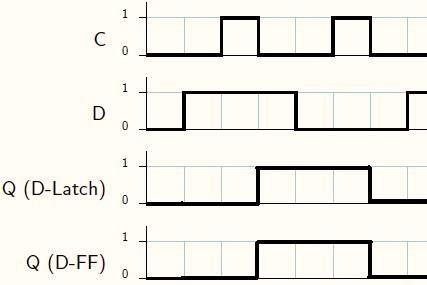
\includegraphics{Impulsdiagramm83a} \\
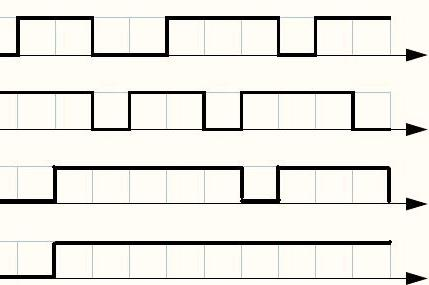
\includegraphics{Impulsdiagramm83b}

\section{Aufgabe 8.4}
\subsection{(a)}

\subsection{(b)}

\subsection{(c)}

\subsection{(d)}

\end{document}
